
\subsection{Some figures}

This is the torsion part of $\THH_*(\ell)$ for $p=3$ and $166 \leq * \leq 317$.
\begin{sidewaysfigure}
  \centering  
  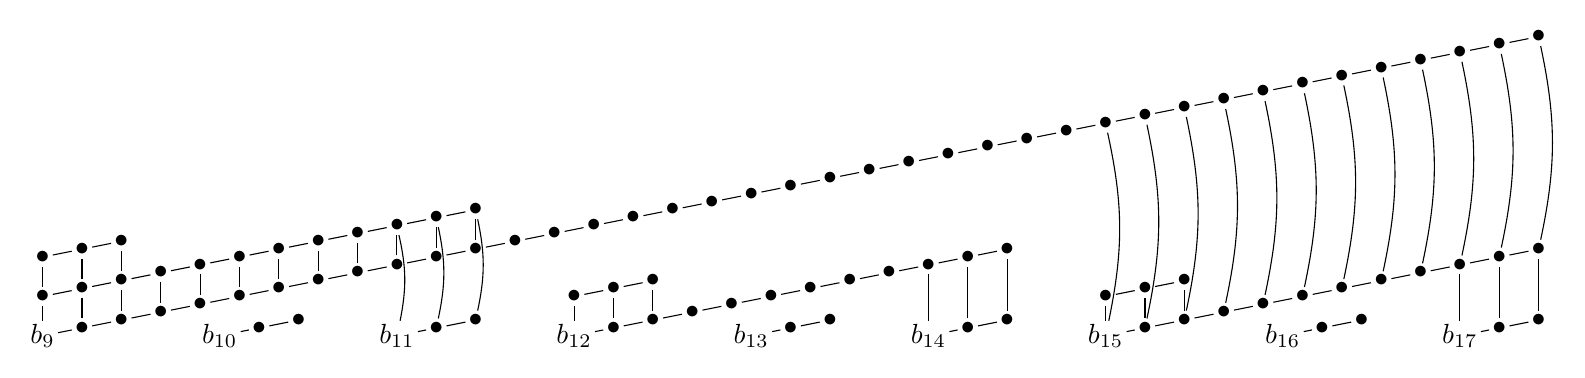
\begin{tikzpicture}[scale = 0.5]
    \node[inner sep = 1pt] (b9v0) at (0.0,0.0) {$b_9$};
    \node[inner sep = 1pt] (b9v1) at (1.0,0.2) {$\bullet$};
    \node[inner sep = 1pt] (b9v2) at (2.0,0.4) {$\bullet$};
    \node[inner sep = 1pt] (b9v3) at (3.0,0.6000000000000001) {$\bullet$};
    \node[inner sep = 1pt] (b9v4) at (4.0,0.8) {$\bullet$};
    \node[inner sep = 1pt] (b9v5) at (5.0,1.0) {$\bullet$};
    \node[inner sep = 1pt] (b9v6) at (6.0,1.2000000000000002) {$\bullet$};
    \node[inner sep = 1pt] (b9v7) at (7.0,1.4000000000000001) {$\bullet$};
    \node[inner sep = 1pt] (b9v8) at (8.0,1.6) {$\bullet$};
    \node[inner sep = 1pt] (b9v9) at (9.0,1.8) {$\bullet$};
    \node[inner sep = 1pt] (b9v10) at (10.0,2.0) {$\bullet$};
    \node[inner sep = 1pt] (b9v11) at (11.0,2.2) {$\bullet$};
    \node[inner sep = 1pt] (b9v12) at (12.0,2.4000000000000004) {$\bullet$};
    \node[inner sep = 1pt] (b9v13) at (13.0,2.6) {$\bullet$};
    \node[inner sep = 1pt] (b9v14) at (14.0,2.8000000000000003) {$\bullet$};
    \node[inner sep = 1pt] (b9v15) at (15.0,3.0) {$\bullet$};
    \node[inner sep = 1pt] (b9v16) at (16.0,3.2) {$\bullet$};
    \node[inner sep = 1pt] (b9v17) at (17.0,3.4000000000000004) {$\bullet$};
    \node[inner sep = 1pt] (b9v18) at (18.0,3.6) {$\bullet$};
    \node[inner sep = 1pt] (b9v19) at (19.0,3.8000000000000003) {$\bullet$};
    \node[inner sep = 1pt] (b9v20) at (20.0,4.0) {$\bullet$};
    \node[inner sep = 1pt] (b9v21) at (21.0,4.2) {$\bullet$};
    \node[inner sep = 1pt] (b9v22) at (22.0,4.4) {$\bullet$};
    \node[inner sep = 1pt] (b9v23) at (23.0,4.6000000000000005) {$\bullet$};
    \node[inner sep = 1pt] (b9v24) at (24.0,4.800000000000001) {$\bullet$};
    \node[inner sep = 1pt] (b9v25) at (25.0,5.0) {$\bullet$};
    \node[inner sep = 1pt] (b9v26) at (26.0,5.2) {$\bullet$};
    \node[inner sep = 1pt] (b9v27) at (27.0,5.4) {$\bullet$};
    \node[inner sep = 1pt] (b9v28) at (28.0,5.6000000000000005) {$\bullet$};
    \node[inner sep = 1pt] (b9v29) at (29.0,5.800000000000001) {$\bullet$};
    \node[inner sep = 1pt] (b9v30) at (30.0,6.0) {$\bullet$};
    \node[inner sep = 1pt] (b9v31) at (31.0,6.2) {$\bullet$};
    \node[inner sep = 1pt] (b9v32) at (32.0,6.4) {$\bullet$};
    \node[inner sep = 1pt] (b9v33) at (33.0,6.6000000000000005) {$\bullet$};
    \node[inner sep = 1pt] (b9v34) at (34.0,6.800000000000001) {$\bullet$};
    \node[inner sep = 1pt] (b9v35) at (35.0,7.0) {$\bullet$};
    \node[inner sep = 1pt] (b9v36) at (36.0,7.2) {$\bullet$};
    \node[inner sep = 1pt] (b9v37) at (37.0,7.4) {$\bullet$};
    \node[inner sep = 1pt] (b9v38) at (38.0,7.6000000000000005) {$\bullet$};

    \draw (b9v0) to (b9v1);
    \draw (b9v1) to (b9v2);
    \draw (b9v2) to (b9v3);
    \draw (b9v3) to (b9v4);
    \draw (b9v4) to (b9v5);
    \draw (b9v5) to (b9v6);
    \draw (b9v6) to (b9v7);
    \draw (b9v7) to (b9v8);
    \draw (b9v8) to (b9v9);
    \draw (b9v9) to (b9v10);
    \draw (b9v10) to (b9v11);
    \draw (b9v11) to (b9v12);
    \draw (b9v12) to (b9v13);
    \draw (b9v13) to (b9v14);
    \draw (b9v14) to (b9v15);
    \draw (b9v15) to (b9v16);
    \draw (b9v16) to (b9v17);
    \draw (b9v17) to (b9v18);
    \draw (b9v18) to (b9v19);
    \draw (b9v19) to (b9v20);
    \draw (b9v20) to (b9v21);
    \draw (b9v21) to (b9v22);
    \draw (b9v22) to (b9v23);
    \draw (b9v23) to (b9v24);
    \draw (b9v24) to (b9v25);
    \draw (b9v25) to (b9v26);
    \draw (b9v26) to (b9v27);
    \draw (b9v27) to (b9v28);
    \draw (b9v28) to (b9v29);
    \draw (b9v29) to (b9v30);
    \draw (b9v30) to (b9v31);
    \draw (b9v31) to (b9v32);
    \draw (b9v32) to (b9v33);
    \draw (b9v33) to (b9v34);
    \draw (b9v34) to (b9v35);
    \draw (b9v35) to (b9v36);
    \draw (b9v36) to (b9v37);
    \draw (b9v37) to (b9v38);

    \node[inner sep = 1pt] (pb9v0) at (0.0,1.0) {$\bullet$};
    \node[inner sep = 1pt] (pb9v1) at (1.0,1.2) {$\bullet$};
    \node[inner sep = 1pt] (pb9v2) at (2.0,1.4) {$\bullet$};
    \node[inner sep = 1pt] (pb9v3) at (3.0,1.6) {$\bullet$};
    \node[inner sep = 1pt] (pb9v4) at (4.0,1.8) {$\bullet$};
    \node[inner sep = 1pt] (pb9v5) at (5.0,2.0) {$\bullet$};
    \node[inner sep = 1pt] (pb9v6) at (6.0,2.2) {$\bullet$};
    \node[inner sep = 1pt] (pb9v7) at (7.0,2.4000000000000004) {$\bullet$};
    \node[inner sep = 1pt] (pb9v8) at (8.0,2.6) {$\bullet$};
    \node[inner sep = 1pt] (pb9v9) at (9.0,2.8) {$\bullet$};
    \node[inner sep = 1pt] (pb9v10) at (10.0,3.0) {$\bullet$};
    \node[inner sep = 1pt] (pb9v11) at (11.0,3.2) {$\bullet$};
    \draw (pb9v0) to (pb9v1);
    \draw (pb9v1) to (pb9v2);
    \draw (pb9v2) to (pb9v3);
    \draw (pb9v3) to (pb9v4);
    \draw (pb9v4) to (pb9v5);
    \draw (pb9v5) to (pb9v6);
    \draw (pb9v6) to (pb9v7);
    \draw (pb9v7) to (pb9v8);
    \draw (pb9v8) to (pb9v9);
    \draw (pb9v9) to (pb9v10);
    \draw (pb9v10) to (pb9v11);

    \draw (b9v0) to (pb9v0);
    \draw (b9v1) to (pb9v1);
    \draw (b9v2) to (pb9v2);
    \draw (b9v3) to (pb9v3);
    \draw (b9v4) to (pb9v4);
    \draw (b9v5) to (pb9v5);
    \draw (b9v6) to (pb9v6);
    \draw (b9v7) to (pb9v7);
    \draw (b9v8) to (pb9v8);
    \draw (b9v9) to (pb9v9);
    \draw (b9v10) to (pb9v10);
    \draw (b9v11) to (pb9v11);

    \node[inner sep = 1pt] (p2b9v0) at (0.0,2.0) {$\bullet$};
    \node[inner sep = 1pt] (p2b9v1) at (1.0,2.2) {$\bullet$};
    \node[inner sep = 1pt] (p2b9v2) at (2.0,2.4) {$\bullet$};
    \draw (p2b9v0) to (p2b9v1);
    \draw (p2b9v1) to (p2b9v2);
    \draw (pb9v0) to (p2b9v0);
    \draw (pb9v1) to (p2b9v1);
    \draw (pb9v2) to (p2b9v2);

    \node[inner sep = 1pt] (b10v0) at (4.5,0.0) {$b_{10}$} ;
    \node[inner sep = 1pt] (b10v1) at (5.5,0.2) {$\bullet$} ;
    \node[inner sep = 1pt] (b10v2) at (6.5,0.4) {$\bullet$} ;
    \draw (b10v0) to (b10v1);
    \draw (b10v1) to (b10v2);

    \node[inner sep = 1pt] (b11v0) at (9.0,0.0) {$b_{11}$} ;
    \node[inner sep = 1pt] (b11v1) at (10.0,0.2) {$\bullet$} ;
    \node[inner sep = 1pt] (b11v2) at (11.0,0.4) {$\bullet$} ;
    \draw (b11v0) to (b11v1);
    \draw (b11v1) to (b11v2);

    \draw (b11v0) to[bend right=12] (pb9v9);
    \draw (b11v1) to[bend right=12] (pb9v10);
    \draw (b11v2) to[bend right=12] (pb9v11);

    \node[inner sep = 1pt] (b12v0) at (13.5,0.0) {$b_{12}$} ;
    \node[inner sep = 1pt] (b12v1) at (14.5,0.2) {$\bullet$} ;
    \node[inner sep = 1pt] (b12v2) at (15.5,0.4) {$\bullet$} ;
    \node[inner sep = 1pt] (b12v3) at (16.5,0.6000000000000001) {$\bullet$} ;
    \node[inner sep = 1pt] (b12v4) at (17.5,0.8) {$\bullet$} ;
    \node[inner sep = 1pt] (b12v5) at (18.5,1.0) {$\bullet$} ;
    \node[inner sep = 1pt] (b12v6) at (19.5,1.2000000000000002) {$\bullet$} ;
    \node[inner sep = 1pt] (b12v7) at (20.5,1.4000000000000001) {$\bullet$} ;
    \node[inner sep = 1pt] (b12v8) at (21.5,1.6) {$\bullet$} ;
    \node[inner sep = 1pt] (b12v9) at (22.5,1.8) {$\bullet$} ;
    \node[inner sep = 1pt] (b12v10) at (23.5,2.0) {$\bullet$} ;
    \node[inner sep = 1pt] (b12v11) at (24.5,2.2) {$\bullet$} ;
    \draw (b12v0) to (b12v1);
    \draw (b12v1) to (b12v2);
    \draw (b12v2) to (b12v3);
    \draw (b12v3) to (b12v4);
    \draw (b12v4) to (b12v5);
    \draw (b12v5) to (b12v6);
    \draw (b12v6) to (b12v7);
    \draw (b12v7) to (b12v8);
    \draw (b12v8) to (b12v9);
    \draw (b12v9) to (b12v10);
    \draw (b12v10) to (b12v11);

    \node[inner sep = 1pt] (pb12v0) at (13.5,1.0) {$\bullet$} ;
    \node[inner sep = 1pt] (pb12v1) at (14.5,1.2) {$\bullet$} ;
    \node[inner sep = 1pt] (pb12v2) at (15.5,1.4) {$\bullet$} ;
    \draw (pb12v0) to (pb12v1);
    \draw (pb12v1) to (pb12v2);

    \draw (b12v0) to (pb12v0);
    \draw (b12v1) to (pb12v1);
    \draw (b12v2) to (pb12v2);

    \node[inner sep = 1pt] (b13v0) at (18.0,0.0) {$b_{13}$} ;
    \node[inner sep = 1pt] (b13v1) at (19.0,0.2) {$\bullet$} ;
    \node[inner sep = 1pt] (b13v2) at (20.0,0.4) {$\bullet$} ;
    \draw (b13v0) to (b13v1);
    \draw (b13v1) to (b13v2);

    \node[inner sep = 1pt] (b14v0) at (22.5,0.0) {$b_{14}$} ;
    \node[inner sep = 1pt] (b14v1) at (23.5,0.2) {$\bullet$} ;
    \node[inner sep = 1pt] (b14v2) at (24.5,0.4) {$\bullet$} ;
    \draw (b14v0) to (b14v1);
    \draw (b14v1) to (b14v2);

    \draw (b14v0) to (b12v9);
    \draw (b14v1) to (b12v10);
    \draw (b14v2) to (b12v11);

    \node[inner sep = 1pt] (b15v0) at (27.0,0.0) {$b_{15}$} ;
    \node[inner sep = 1pt] (b15v1) at (28.0,0.2) {$\bullet$} ;
    \node[inner sep = 1pt] (b15v2) at (29.0,0.4) {$\bullet$} ;
    \node[inner sep = 1pt] (b15v3) at (30.0,0.6000000000000001) {$\bullet$} ;
    \node[inner sep = 1pt] (b15v4) at (31.0,0.8) {$\bullet$} ;
    \node[inner sep = 1pt] (b15v5) at (32.0,1.0) {$\bullet$} ;
    \node[inner sep = 1pt] (b15v6) at (33.0,1.2000000000000002) {$\bullet$} ;
    \node[inner sep = 1pt] (b15v7) at (34.0,1.4000000000000001) {$\bullet$} ;
    \node[inner sep = 1pt] (b15v8) at (35.0,1.6) {$\bullet$} ;
    \node[inner sep = 1pt] (b15v9) at (36.0,1.8) {$\bullet$} ;
    \node[inner sep = 1pt] (b15v10) at (37.0,2.0) {$\bullet$} ;
    \node[inner sep = 1pt] (b15v11) at (38.0,2.2) {$\bullet$} ;
    \draw (b15v0) to (b15v1);
    \draw (b15v1) to (b15v2);
    \draw (b15v2) to (b15v3);
    \draw (b15v3) to (b15v4);
    \draw (b15v4) to (b15v5);
    \draw (b15v5) to (b15v6);
    \draw (b15v6) to (b15v7);
    \draw (b15v7) to (b15v8);
    \draw (b15v8) to (b15v9);
    \draw (b15v9) to (b15v10);
    \draw (b15v10) to (b15v11);

    \node[inner sep = 1pt] (pb15v0) at (27.0,1.0) {$\bullet$} ;
    \node[inner sep = 1pt] (pb15v1) at (28.0,1.2) {$\bullet$} ;
    \node[inner sep = 1pt] (pb15v2) at (29.0,1.4) {$\bullet$} ;
    \draw (pb15v0) to (pb15v1);
    \draw (pb15v1) to (pb15v2);

    \draw (b15v0) to (pb15v0);
    \draw (b15v1) to (pb15v1);
    \draw (b15v2) to (pb15v2);

    \draw[bend right = 12] (b15v0) to (b9v27);
    \draw[bend right = 12] (b15v1) to (b9v28);
    \draw[bend right = 12] (b15v2) to (b9v29);
    \draw[bend right = 12] (b15v3) to (b9v30);
    \draw[bend right = 12] (b15v4) to (b9v31);
    \draw[bend right = 12] (b15v5) to (b9v32);
    \draw[bend right = 12] (b15v6) to (b9v33);
    \draw[bend right = 12] (b15v7) to (b9v34);
    \draw[bend right = 12] (b15v8) to (b9v35);
    \draw[bend right = 12] (b15v9) to (b9v36);
    \draw[bend right = 12] (b15v10) to (b9v37);
    \draw[bend right = 12] (b15v11) to (b9v38);

    \node[inner sep = 1pt] (b16v0) at (31.5,0.0) {$b_{16}$} ;
    \node[inner sep = 1pt] (b16v1) at (32.5,0.2) {$\bullet$} ;
    \node[inner sep = 1pt] (b16v2) at (33.5,0.4) {$\bullet$} ;
    \draw (b16v0) to (b16v1);
    \draw (b16v1) to (b16v2);

    \node[inner sep = 1pt] (b17v0) at (36.0,0.0) {$b_{17}$} ;
    \node[inner sep = 1pt] (b17v1) at (37.0,0.2) {$\bullet$} ;
    \node[inner sep = 1pt] (b17v2) at (38.0,0.4) {$\bullet$} ;
    \draw (b17v0) to (b17v1);
    \draw (b17v1) to (b17v2);

    \draw (b17v0) to (b15v9);
    \draw (b17v1) to (b15v10);
    \draw (b17v2) to (b15v11);
  \end{tikzpicture}
  \label{fig:thhell1}
  \caption{Torsion part of $\THH_*(\ell)$ for $p=3$ and $166 \leq * \leq 317$.}
\end{sidewaysfigure}

Figure \ref{fig:thhbpell1} is what is left in the $E^\infty$-page of the spectral sequence
\begin{equation}
  \THH_*(\ell)\langle \sigma v_2 \rangle \Rightarrow \THH_*(\BP \langle 2 \rangle; \ell)
\end{equation}
in the source of $\partial$. Figure \ref{fig:thhbpell2} is what is left in the image of $\partial$, that is the copy of $\THH_*(\ell)$ multiplied by $\sigma v_2$.


\begin{sidewaysfigure}
  \centering
    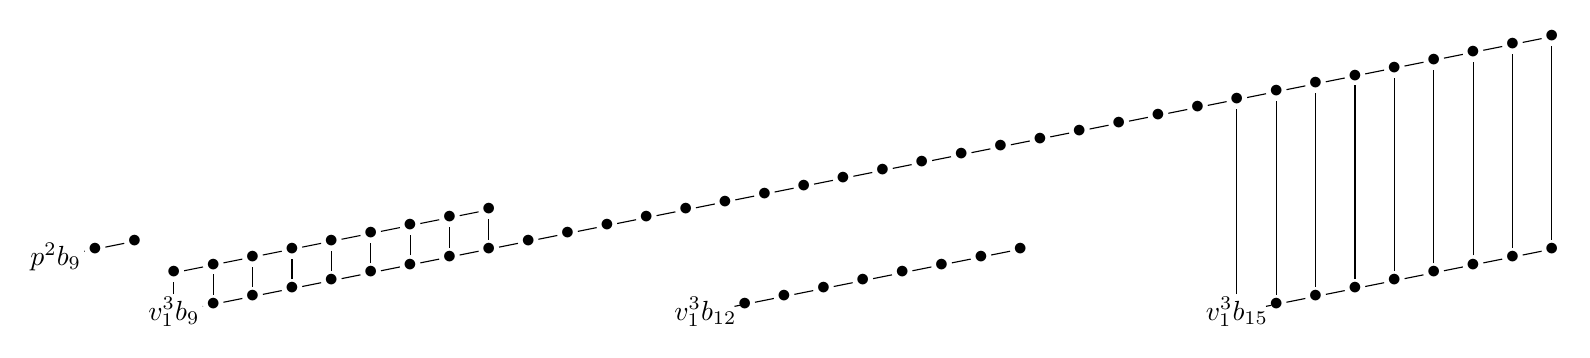
\begin{tikzpicture}[scale = 0.5]
    \node[inner sep = 1pt] (b9v3) at (3.0,0.6000000000000001) {$v_1^3b_{9}$};
    \node[inner sep = 1pt] (b9v4) at (4.0,0.8) {$\bullet$};
    \node[inner sep = 1pt] (b9v5) at (5.0,1.0) {$\bullet$};
    \node[inner sep = 1pt] (b9v6) at (6.0,1.2000000000000002) {$\bullet$};
    \node[inner sep = 1pt] (b9v7) at (7.0,1.4000000000000001) {$\bullet$};
    \node[inner sep = 1pt] (b9v8) at (8.0,1.6) {$\bullet$};
    \node[inner sep = 1pt] (b9v9) at (9.0,1.8) {$\bullet$};
    \node[inner sep = 1pt] (b9v10) at (10.0,2.0) {$\bullet$};
    \node[inner sep = 1pt] (b9v11) at (11.0,2.2) {$\bullet$};
    \node[inner sep = 1pt] (b9v12) at (12.0,2.4000000000000004) {$\bullet$};
    \node[inner sep = 1pt] (b9v13) at (13.0,2.6) {$\bullet$};
    \node[inner sep = 1pt] (b9v14) at (14.0,2.8000000000000003) {$\bullet$};
    \node[inner sep = 1pt] (b9v15) at (15.0,3.0) {$\bullet$};
    \node[inner sep = 1pt] (b9v16) at (16.0,3.2) {$\bullet$};
    \node[inner sep = 1pt] (b9v17) at (17.0,3.4000000000000004) {$\bullet$};
    \node[inner sep = 1pt] (b9v18) at (18.0,3.6) {$\bullet$};
    \node[inner sep = 1pt] (b9v19) at (19.0,3.8000000000000003) {$\bullet$};
    \node[inner sep = 1pt] (b9v20) at (20.0,4.0) {$\bullet$};
    \node[inner sep = 1pt] (b9v21) at (21.0,4.2) {$\bullet$};
    \node[inner sep = 1pt] (b9v22) at (22.0,4.4) {$\bullet$};
    \node[inner sep = 1pt] (b9v23) at (23.0,4.6000000000000005) {$\bullet$};
    \node[inner sep = 1pt] (b9v24) at (24.0,4.800000000000001) {$\bullet$};
    \node[inner sep = 1pt] (b9v25) at (25.0,5.0) {$\bullet$};
    \node[inner sep = 1pt] (b9v26) at (26.0,5.2) {$\bullet$};
    \node[inner sep = 1pt] (b9v27) at (27.0,5.4) {$\bullet$};
    \node[inner sep = 1pt] (b9v28) at (28.0,5.6000000000000005) {$\bullet$};
    \node[inner sep = 1pt] (b9v29) at (29.0,5.800000000000001) {$\bullet$};
    \node[inner sep = 1pt] (b9v30) at (30.0,6.0) {$\bullet$};
    \node[inner sep = 1pt] (b9v31) at (31.0,6.2) {$\bullet$};
    \node[inner sep = 1pt] (b9v32) at (32.0,6.4) {$\bullet$};
    \node[inner sep = 1pt] (b9v33) at (33.0,6.6000000000000005) {$\bullet$};
    \node[inner sep = 1pt] (b9v34) at (34.0,6.800000000000001) {$\bullet$};
    \node[inner sep = 1pt] (b9v35) at (35.0,7.0) {$\bullet$};
    \node[inner sep = 1pt] (b9v36) at (36.0,7.2) {$\bullet$};
    \node[inner sep = 1pt] (b9v37) at (37.0,7.4) {$\bullet$};
    \node[inner sep = 1pt] (b9v38) at (38.0,7.6000000000000005) {$\bullet$};

    \draw (b9v3) to (b9v4);
    \draw (b9v4) to (b9v5);
    \draw (b9v5) to (b9v6);
    \draw (b9v6) to (b9v7);
    \draw (b9v7) to (b9v8);
    \draw (b9v8) to (b9v9);
    \draw (b9v9) to (b9v10);
    \draw (b9v10) to (b9v11);
    \draw (b9v11) to (b9v12);
    \draw (b9v12) to (b9v13);
    \draw (b9v13) to (b9v14);
    \draw (b9v14) to (b9v15);
    \draw (b9v15) to (b9v16);
    \draw (b9v16) to (b9v17);
    \draw (b9v17) to (b9v18);
    \draw (b9v18) to (b9v19);
    \draw (b9v19) to (b9v20);
    \draw (b9v20) to (b9v21);
    \draw (b9v21) to (b9v22);
    \draw (b9v22) to (b9v23);
    \draw (b9v23) to (b9v24);
    \draw (b9v24) to (b9v25);
    \draw (b9v25) to (b9v26);
    \draw (b9v26) to (b9v27);
    \draw (b9v27) to (b9v28);
    \draw (b9v28) to (b9v29);
    \draw (b9v29) to (b9v30);
    \draw (b9v30) to (b9v31);
    \draw (b9v31) to (b9v32);
    \draw (b9v32) to (b9v33);
    \draw (b9v33) to (b9v34);
    \draw (b9v34) to (b9v35);
    \draw (b9v35) to (b9v36);
    \draw (b9v36) to (b9v37);
    \draw (b9v37) to (b9v38);

    \node[inner sep = 1pt] (pb9v3) at (3.0,1.6) {$\bullet$};
    \node[inner sep = 1pt] (pb9v4) at (4.0,1.8) {$\bullet$};
    \node[inner sep = 1pt] (pb9v5) at (5.0,2.0) {$\bullet$};
    \node[inner sep = 1pt] (pb9v6) at (6.0,2.2) {$\bullet$};
    \node[inner sep = 1pt] (pb9v7) at (7.0,2.4000000000000004) {$\bullet$};
    \node[inner sep = 1pt] (pb9v8) at (8.0,2.6) {$\bullet$};
    \node[inner sep = 1pt] (pb9v9) at (9.0,2.8) {$\bullet$};
    \node[inner sep = 1pt] (pb9v10) at (10.0,3.0) {$\bullet$};
    \node[inner sep = 1pt] (pb9v11) at (11.0,3.2) {$\bullet$};
    \draw (pb9v3) to (pb9v4);
    \draw (pb9v4) to (pb9v5);
    \draw (pb9v5) to (pb9v6);
    \draw (pb9v6) to (pb9v7);
    \draw (pb9v7) to (pb9v8);
    \draw (pb9v8) to (pb9v9);
    \draw (pb9v9) to (pb9v10);
    \draw (pb9v10) to (pb9v11);

    \draw (b9v3) to (pb9v3);
    \draw (b9v4) to (pb9v4);
    \draw (b9v5) to (pb9v5);
    \draw (b9v6) to (pb9v6);
    \draw (b9v7) to (pb9v7);
    \draw (b9v8) to (pb9v8);
    \draw (b9v9) to (pb9v9);
    \draw (b9v10) to (pb9v10);
    \draw (b9v11) to (pb9v11);

    \node[inner sep = 1pt] (p2b9v0) at (0.0,2.0) {$p^2b_9$};
    \node[inner sep = 1pt] (p2b9v1) at (1.0,2.2) {$\bullet$};
    \node[inner sep = 1pt] (p2b9v2) at (2.0,2.4) {$\bullet$};
    \draw (p2b9v0) to (p2b9v1);
    \draw (p2b9v1) to (p2b9v2);
    
    \node[inner sep = 1pt] (b12v3) at (16.5,0.6000000000000001) {$v_1^3b_{12}$} ;
    \node[inner sep = 1pt] (b12v4) at (17.5,0.8) {$\bullet$} ;
    \node[inner sep = 1pt] (b12v5) at (18.5,1.0) {$\bullet$} ;
    \node[inner sep = 1pt] (b12v6) at (19.5,1.2000000000000002) {$\bullet$} ;
    \node[inner sep = 1pt] (b12v7) at (20.5,1.4000000000000001) {$\bullet$} ;
    \node[inner sep = 1pt] (b12v8) at (21.5,1.6) {$\bullet$} ;
    \node[inner sep = 1pt] (b12v9) at (22.5,1.8) {$\bullet$} ;
    \node[inner sep = 1pt] (b12v10) at (23.5,2.0) {$\bullet$} ;
    \node[inner sep = 1pt] (b12v11) at (24.5,2.2) {$\bullet$} ;
    \draw (b12v3) to (b12v4);
    \draw (b12v4) to (b12v5);
    \draw (b12v5) to (b12v6);
    \draw (b12v6) to (b12v7);
    \draw (b12v7) to (b12v8);
    \draw (b12v8) to (b12v9);
    \draw (b12v9) to (b12v10);
    \draw (b12v10) to (b12v11);

    \node[inner sep = 1pt] (b15v3) at (30.0,0.6000000000000001) {$v_1^3b_{15}$} ;
    \node[inner sep = 1pt] (b15v4) at (31.0,0.8) {$\bullet$} ;
    \node[inner sep = 1pt] (b15v5) at (32.0,1.0) {$\bullet$} ;
    \node[inner sep = 1pt] (b15v6) at (33.0,1.2000000000000002) {$\bullet$} ;
    \node[inner sep = 1pt] (b15v7) at (34.0,1.4000000000000001) {$\bullet$} ;
    \node[inner sep = 1pt] (b15v8) at (35.0,1.6) {$\bullet$} ;
    \node[inner sep = 1pt] (b15v9) at (36.0,1.8) {$\bullet$} ;
    \node[inner sep = 1pt] (b15v10) at (37.0,2.0) {$\bullet$} ;
    \node[inner sep = 1pt] (b15v11) at (38.0,2.2) {$\bullet$} ;
    \draw (b15v3) to (b15v4);
    \draw (b15v4) to (b15v5);
    \draw (b15v5) to (b15v6);
    \draw (b15v6) to (b15v7);
    \draw (b15v7) to (b15v8);
    \draw (b15v8) to (b15v9);
    \draw (b15v9) to (b15v10);
    \draw (b15v10) to (b15v11);

    \draw (b15v3) to (b9v30);
    \draw (b15v4) to (b9v31);
    \draw (b15v5) to (b9v32);
    \draw (b15v6) to (b9v33);
    \draw (b15v7) to (b9v34);
    \draw (b15v8) to (b9v35);
    \draw (b15v9) to (b9v36);
    \draw (b15v10) to (b9v37);
    \draw (b15v11) to (b9v38);
  \end{tikzpicture}
  \label{fig:thhbpell1}
  \caption{$E^\infty$-page, generated by 1 part}
\end{sidewaysfigure}


\begin{sidewaysfigure}
  \centering  
  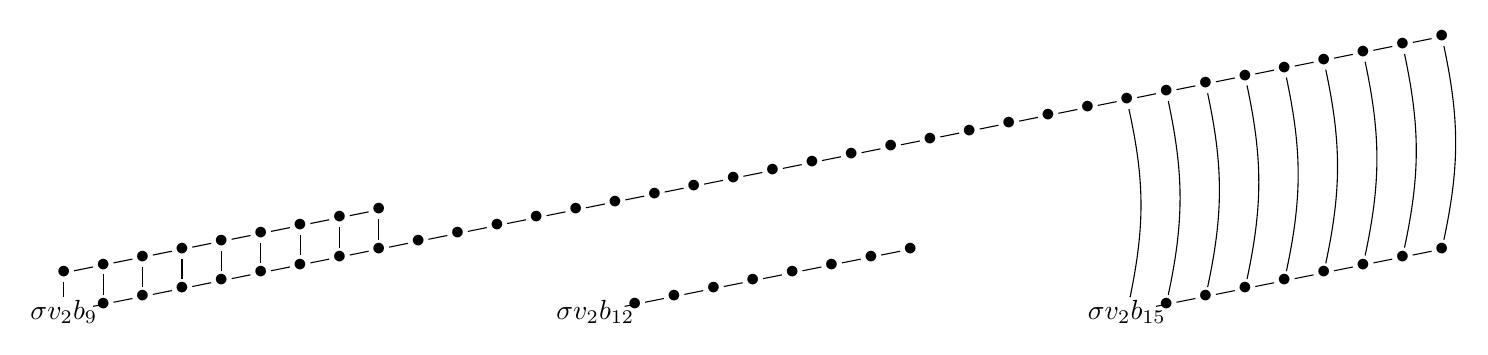
\begin{tikzpicture}[scale = 0.5]
    \node[inner sep = 1pt] (b9v0) at (0.0,0.0) {$\sigma v_2 b_9$};
    \node[inner sep = 1pt] (b9v1) at (1.0,0.2) {$\bullet$};
    \node[inner sep = 1pt] (b9v2) at (2.0,0.4) {$\bullet$};
    \node[inner sep = 1pt] (b9v3) at (3.0,0.6000000000000001) {$\bullet$};
    \node[inner sep = 1pt] (b9v4) at (4.0,0.8) {$\bullet$};
    \node[inner sep = 1pt] (b9v5) at (5.0,1.0) {$\bullet$};
    \node[inner sep = 1pt] (b9v6) at (6.0,1.2000000000000002) {$\bullet$};
    \node[inner sep = 1pt] (b9v7) at (7.0,1.4000000000000001) {$\bullet$};
    \node[inner sep = 1pt] (b9v8) at (8.0,1.6) {$\bullet$};
    \node[inner sep = 1pt] (b9v9) at (9.0,1.8) {$\bullet$};
    \node[inner sep = 1pt] (b9v10) at (10.0,2.0) {$\bullet$};
    \node[inner sep = 1pt] (b9v11) at (11.0,2.2) {$\bullet$};
    \node[inner sep = 1pt] (b9v12) at (12.0,2.4000000000000004) {$\bullet$};
    \node[inner sep = 1pt] (b9v13) at (13.0,2.6) {$\bullet$};
    \node[inner sep = 1pt] (b9v14) at (14.0,2.8000000000000003) {$\bullet$};
    \node[inner sep = 1pt] (b9v15) at (15.0,3.0) {$\bullet$};
    \node[inner sep = 1pt] (b9v16) at (16.0,3.2) {$\bullet$};
    \node[inner sep = 1pt] (b9v17) at (17.0,3.4000000000000004) {$\bullet$};
    \node[inner sep = 1pt] (b9v18) at (18.0,3.6) {$\bullet$};
    \node[inner sep = 1pt] (b9v19) at (19.0,3.8000000000000003) {$\bullet$};
    \node[inner sep = 1pt] (b9v20) at (20.0,4.0) {$\bullet$};
    \node[inner sep = 1pt] (b9v21) at (21.0,4.2) {$\bullet$};
    \node[inner sep = 1pt] (b9v22) at (22.0,4.4) {$\bullet$};
    \node[inner sep = 1pt] (b9v23) at (23.0,4.6000000000000005) {$\bullet$};
    \node[inner sep = 1pt] (b9v24) at (24.0,4.800000000000001) {$\bullet$};
    \node[inner sep = 1pt] (b9v25) at (25.0,5.0) {$\bullet$};
    \node[inner sep = 1pt] (b9v26) at (26.0,5.2) {$\bullet$};
    \node[inner sep = 1pt] (b9v27) at (27.0,5.4) {$\bullet$};
    \node[inner sep = 1pt] (b9v28) at (28.0,5.6000000000000005) {$\bullet$};
    \node[inner sep = 1pt] (b9v29) at (29.0,5.800000000000001) {$\bullet$};
    \node[inner sep = 1pt] (b9v30) at (30.0,6.0) {$\bullet$};
    \node[inner sep = 1pt] (b9v31) at (31.0,6.2) {$\bullet$};
    \node[inner sep = 1pt] (b9v32) at (32.0,6.4) {$\bullet$};
    \node[inner sep = 1pt] (b9v33) at (33.0,6.6000000000000005) {$\bullet$};
    \node[inner sep = 1pt] (b9v34) at (34.0,6.800000000000001) {$\bullet$};
    \node[inner sep = 1pt] (b9v35) at (35.0,7.0) {$\bullet$};

    \draw (b9v0) to (b9v1);
    \draw (b9v1) to (b9v2);
    \draw (b9v2) to (b9v3);
    \draw (b9v3) to (b9v4);
    \draw (b9v4) to (b9v5);
    \draw (b9v5) to (b9v6);
    \draw (b9v6) to (b9v7);
    \draw (b9v7) to (b9v8);
    \draw (b9v8) to (b9v9);
    \draw (b9v9) to (b9v10);
    \draw (b9v10) to (b9v11);
    \draw (b9v11) to (b9v12);
    \draw (b9v12) to (b9v13);
    \draw (b9v13) to (b9v14);
    \draw (b9v14) to (b9v15);
    \draw (b9v15) to (b9v16);
    \draw (b9v16) to (b9v17);
    \draw (b9v17) to (b9v18);
    \draw (b9v18) to (b9v19);
    \draw (b9v19) to (b9v20);
    \draw (b9v20) to (b9v21);
    \draw (b9v21) to (b9v22);
    \draw (b9v22) to (b9v23);
    \draw (b9v23) to (b9v24);
    \draw (b9v24) to (b9v25);
    \draw (b9v25) to (b9v26);
    \draw (b9v26) to (b9v27);
    \draw (b9v27) to (b9v28);
    \draw (b9v28) to (b9v29);
    \draw (b9v29) to (b9v30);
    \draw (b9v30) to (b9v31);
    \draw (b9v31) to (b9v32);
    \draw (b9v32) to (b9v33);
    \draw (b9v33) to (b9v34);
    \draw (b9v34) to (b9v35);

    \node[inner sep = 1pt] (pb9v0) at (0.0,1.0) {$\bullet$};
    \node[inner sep = 1pt] (pb9v1) at (1.0,1.2) {$\bullet$};
    \node[inner sep = 1pt] (pb9v2) at (2.0,1.4) {$\bullet$};
    \node[inner sep = 1pt] (pb9v3) at (3.0,1.6) {$\bullet$};
    \node[inner sep = 1pt] (pb9v4) at (4.0,1.8) {$\bullet$};
    \node[inner sep = 1pt] (pb9v5) at (5.0,2.0) {$\bullet$};
    \node[inner sep = 1pt] (pb9v6) at (6.0,2.2) {$\bullet$};
    \node[inner sep = 1pt] (pb9v7) at (7.0,2.4000000000000004) {$\bullet$};
    \node[inner sep = 1pt] (pb9v8) at (8.0,2.6) {$\bullet$};
    \draw (pb9v0) to (pb9v1);
    \draw (pb9v1) to (pb9v2);
    \draw (pb9v2) to (pb9v3);
    \draw (pb9v3) to (pb9v4);
    \draw (pb9v4) to (pb9v5);
    \draw (pb9v5) to (pb9v6);
    \draw (pb9v6) to (pb9v7);
    \draw (pb9v7) to (pb9v8);

    \draw (b9v0) to (pb9v0);
    \draw (b9v1) to (pb9v1);
    \draw (b9v2) to (pb9v2);
    \draw (b9v3) to (pb9v3);
    \draw (b9v4) to (pb9v4);
    \draw (b9v5) to (pb9v5);
    \draw (b9v6) to (pb9v6);
    \draw (b9v7) to (pb9v7);
    \draw (b9v8) to (pb9v8);

    \node[inner sep = 1pt] (b12v0) at (13.5,0.0) {$\sigma v_2 b_{12}$} ;
    \node[inner sep = 1pt] (b12v1) at (14.5,0.2) {$\bullet$} ;
    \node[inner sep = 1pt] (b12v2) at (15.5,0.4) {$\bullet$} ;
    \node[inner sep = 1pt] (b12v3) at (16.5,0.6000000000000001) {$\bullet$} ;
    \node[inner sep = 1pt] (b12v4) at (17.5,0.8) {$\bullet$} ;
    \node[inner sep = 1pt] (b12v5) at (18.5,1.0) {$\bullet$} ;
    \node[inner sep = 1pt] (b12v6) at (19.5,1.2000000000000002) {$\bullet$} ;
    \node[inner sep = 1pt] (b12v7) at (20.5,1.4000000000000001) {$\bullet$} ;
    \node[inner sep = 1pt] (b12v8) at (21.5,1.6) {$\bullet$} ;
    \draw (b12v0) to (b12v1);
    \draw (b12v1) to (b12v2);
    \draw (b12v2) to (b12v3);
    \draw (b12v3) to (b12v4);
    \draw (b12v4) to (b12v5);
    \draw (b12v5) to (b12v6);
    \draw (b12v6) to (b12v7);
    \draw (b12v7) to (b12v8);
    
    \node[inner sep = 1pt] (b15v0) at (27.0,0.0) {$\sigma v_2 b_{15}$} ;
    \node[inner sep = 1pt] (b15v1) at (28.0,0.2) {$\bullet$} ;
    \node[inner sep = 1pt] (b15v2) at (29.0,0.4) {$\bullet$} ;
    \node[inner sep = 1pt] (b15v3) at (30.0,0.6000000000000001) {$\bullet$} ;
    \node[inner sep = 1pt] (b15v4) at (31.0,0.8) {$\bullet$} ;
    \node[inner sep = 1pt] (b15v5) at (32.0,1.0) {$\bullet$} ;
    \node[inner sep = 1pt] (b15v6) at (33.0,1.2000000000000002) {$\bullet$} ;
    \node[inner sep = 1pt] (b15v7) at (34.0,1.4000000000000001) {$\bullet$} ;
    \node[inner sep = 1pt] (b15v8) at (35.0,1.6) {$\bullet$} ;
    \draw (b15v0) to (b15v1);
    \draw (b15v1) to (b15v2);
    \draw (b15v2) to (b15v3);
    \draw (b15v3) to (b15v4);
    \draw (b15v4) to (b15v5);
    \draw (b15v5) to (b15v6);
    \draw (b15v6) to (b15v7);
    \draw (b15v7) to (b15v8);

    \draw[bend right = 12] (b15v0) to (b9v27);
    \draw[bend right = 12] (b15v1) to (b9v28);
    \draw[bend right = 12] (b15v2) to (b9v29);
    \draw[bend right = 12] (b15v3) to (b9v30);
    \draw[bend right = 12] (b15v4) to (b9v31);
    \draw[bend right = 12] (b15v5) to (b9v32);
    \draw[bend right = 12] (b15v6) to (b9v33);
    \draw[bend right = 12] (b15v7) to (b9v34);
    \draw[bend right = 12] (b15v8) to (b9v35);
  \end{tikzpicture}
  \label{fig:thhbpell2}
  \caption{$E^\infty$-page, generated by $\sigma v_2$ part}
\end{sidewaysfigure}
